\chapter{Mobile manipulation system design}
\label{cha:mmsdesign}

%---------------------------------------------------------------------------

\section{Project background}
\label{sec:background}

A mobile manipulation system (MMS) is a robotic system that is capable of both manipulating objects and locomotion. Typically, the system is composed of a robotic arm based on a robotic mobile platform. Such configuration enables the manipulator to operate in an unlimited workspace, thus providing great application opportunities.

Typically, mobile manipulators are designed to relieve people in hostile situations. They are, for example, widely used in the field of chemical, biological, radioactive or nuclear (CBRN) defense. Explosive materials and other hazardous substances can be disposed without exposing operators to any danger. Another example is space exploration, where manipulation systems are used in planetary rovers in unmanned exploratory missions on other planets. Substitution of human operators in such expeditions significantly reduce their expenditure and risk.

Augmenting the MMS design with a certain degree of autonomy, brings the possibility for the robot to be used as a human-assistant in the household. Most of current applications in this field refer to pick up and delivery services, that have the potential to improve lives of the elderly, injured and disabled people []. Furthermore, typical service robots in human environments are dedicated to accomplish only a single task, such as vacuum cleaning, lawn mowing, pool cleaning or window washing. Their operation is achieved by adjusting existing domestic appliances with a degree of autonomy. With a multi purpose robotic system such as a mobile manipulator, it is potentially possible not to replace existing devices but to substitute the human operator. 

Autonomous gripping and transportation with a MMS could also be used in the industry for designing flexible factory plants and intelligent warehouses []. A manufacturing process that utilizes the MMS robots is simpler and more cost effective in adapting to the market changes. The production could be more customized by applying MMS robots in transportation, preparatory and post-processing tasks. Furthermore, even the most advanced distribution centres, such as the Amazon Kiva Systems [kiva?], require repetitive human work to manipulate goods in the unstructured environment. Therefore, the warehousing process could benefit by applying autonomous MMS robots and there are ongoing efforts in this area [amazonchallenge].

% www.willowgarage.com/pages/pr2/overview

One of the most promising applications of MMS is the PR2 development platform from the Willow Garage company. PR2 is a human-sized robot, equipped with two 7 degree-of-freedom manipulators, omnidirectional mobile base, a processing power of two Xeon servers with 8 cores and 24GB of RAM each, and a multitude of sensors, including stereo, time-of flight and structured light cameras, LIDAR scanners, and an inertial measurement unit [prspecs]. The PR2 robot has already proven successful in such dexterous experiments as opening doors, playing pool, folding towels and serving beverages to people[prapps]. 

Wide functionality of a MMS robot makes its design a challenging task. In MMS robots, the unstructured environment and additional degrees of freedom complicate the control task. Furthermore, the workspace of a manipulator is often shared with people and other vehicles. Such work environment renders many potentially hazardous situations. Therefore, it requires a highly sophisticated control system, with vision based feedback. 

%---------------------------------------------------------------------------

\section{Design requirements}
\label{sec:require}

In order to clarify the design process, the requirements that should be met by the final construction were defined. The main goals and features of the project are summarized in the following list:

\begin{enumerate}
\item The robotic system should consist of two cooperating serial manipulators, based on a common mobile robotic platform.
\item The whole construction should be assembled from easily accessible components, available on the consumer market.
\item The serial manipulators should be equipped with grippers for general object manipulation.
\item The manipulators reachable workspace should allow to reach objects located on the ground.
\item The reachable workspace of each manipulator should also intersect, to allow collaboration on manipulation tasks.
\item The mobile platform should be wheeled and is expected to move only on flat surfaces at indoor areas.
\item The steering mechanism of the robot chassis should be kept simple and convenient to control.
\item The robotic system is expected to provide an interface for remote control, developed in a commonly used and well supported standard.
\item The control interface of the robot is required to provide methods for manipulator joints positioning and for setting velocity and direction of the platform movement. 
\item The whole system should be powered by a source that could withstand at least an hour of continuous work.
\end{enumerate}

Furthermore, as the robot is intended for autonomous operation, it should possess a vision based data acquisition system and a computing unit with enough processing power to analyse the acquired data in an online fashion.

\begin{comment}
In robotics a serial manipulator is a device used to manipulate objects. It consists of a kinematic chain with actuated joints. The type of the joint can be prismatic or revolute, correspondingly allowing for either rotational or transational motion. The last link of the chain is called an end-effector, which is used to interact with the environment.
 
 
 Robotic arm reachable workspace is defined as a set of points at which end-effector can be located. Manipulators are usually classified by their structural configuration, that is, the type of first three joints in the kinematic chain. We distignuish four basic types of such configuration: 

\begin{enumerate}
\item Cartesian - three prismatic joints \textcolor{red}{pros/cons}
\item Cylindrical - two prismatic and one revolute joints \textcolor{red}{pros/cons}
\item Spherical - one prismatic and two revolute joints  \textcolor{red}{pros/cons}
\item Articulated - three revolute joints  \textcolor{red}{often called antromorphic, since it mimics human arm structure. It provides relatively large workspace and is convinient for obstacle avoidance, although it is the most difficult in positioning. }
\end{enumerate}

 For every manipulator, the position and orientation of its end-effector can be derived from its joint positions and its geometric model. The inverse problem however, is more difficult and does not always have a solution. In 1968 Donald L. Peiper showed that \textit{the inverse kinematics of serial manipulators with six revolute joints, and with three consecutive joints intersecting, can be solved in closed-form, i.e. analytically}. This result is referred to as \textcolor{red}{321 kinematic structure []}, since the three wrist joints intersect, the two shoulder and elbow joints are parallel, and the first joint orthogonally intersects the first shoulder joint. The 321 design is an example of a 6R wrist-partitioned manipulator, which is one the most widely used type of manipulator in the industry.
 
 Modern industrial robotic arms are characterized with high precision and repeatability. They usually work in a fixed workspace, on factory plants, where they relieve humans from repeatable, dull and often dangerous tasks.\textcolor{red}{ On the other hand, limited workspace of a manipulator imposes high costs of any changes in the manufacturing process. Inflexibility of the plant to different products [].}


Generally speaking, a mobile robotic platform is an automatic machine that is capable of locomotion. Movement of a robot can be achieved in various ways, such as walking, rolling, hopping, metachronal motion etc. In general, wheeled robots consume less energy than other locomotion mechanisms. [1] The most crucial aspect of design in such robots is the type of used wheel. Standard wheels, although simple in structure and good in reliability, impose nonholonomic velocity constraints that limit robot motion. On the other hand, there are special wheel designs, with which a robot can obtain omnidirectional motion, removing those constraints. Mecanum wheels are an example of such wheels. They were invented in 1973 by Bengt Ilon, an engineer in Swedish company Mecanum AB [2]. In principle, they are composed of a central wheel with a set of rollers attached on its periphery at a certain angle. Depending on each individual wheels direction and speed, the total force vector can be achieved in any desired direction, ensuring three degrees of freedom for planar motion of the whole platform. [3]


A mobile manipulator is a robotic system composed of a mobile platform and a robotic arm. Combining locomotion with manipulation enables the manipulator to operate in unlimited workspace, which makes it more flexible and provides great application possibilities. On the other hand, such design considerably complicates the control task. Due to additional degrees of freedom and unstructured environment, additional systems need to be introduced. A robot of that kind requires simultaneous navigation, path planning, object recognition and manipulation. Workspace of a mobile manipulator is usually shared with people and other vehicles, which render many potentially hazardous situations and impose entirely new and high demands on the security system. Addressing those problems have already been widely discussed in the literature, for example in [8][9][10].

Mobile manipulation requires a data acquisition system with a variety of sensors to collect information about the environment and accomplish its tasks. Navigational information for dead reckoning task is usually gathered by odometry sensors, inertial units, and sometimes by RF position-location systems. Typically, tactile bumpers and ultrasonic or infrared proximity sensors provide necessary data to solve collision avoidance problems. Stereo-cameras, time-of-flight cameras, laser LIDARs and RGB-D sensors are generally utilised in vision systems resolving tasks such as object recognition and pose estimation. A vision system that provides depth information can also serve as a collision avoidance system or may navigate the robot.

%---------

The MPTM robot consists of two robotic arms based on a simple four-wheeled mobile platform. Both of robotic arms have 5 degrees of freedom and are in articulated structural configuration. To avoid complicating the mechanical design of the chassis with a steering mechanism, a special kind of wheels were used. Mecanum wheels, as they are called, are equipped with a set of rollers attached to their circumference, which allow a vehicle to move in any direction without turning the wheels. 

By alternating wheels with left and right-handed rollers, in such a way that each wheel applies force roughly at right angles to the wheelbase diagonal the wheel is on, the vehicle is stable and can be made to move in any direction and turn by varying the speed and direction of rotation of each wheel. Moving all four wheels in the same direction causes forward or backward movement, running the wheels on one side in the opposite direction to those on the other side causes rotation of the vehicle, and running the wheels on one diagonal in the opposite direction to those on the other diagonal causes sideways movement. Combinations of these wheel motions allow for vehicle motion in any direction with any vehicle rotation.

Another advantage of such design is increased stability of the platform.

The MPTM robot utilises two types of actuators, 4 DC motors for the mobile platform wheels and 12 servomechanisms for manipulator joints. 
All DC motors have 50:1 metal gearboxes. They achieve 200 RPM of no-load speed and 12 kg cm of stall current. Additionally, they possess 64 CPR encoders, which multiplied by the gear ratio provide 3200 counts per revolution.

Servomechanisms used are Turnigy 1269HV, with operating speed of 

Actuators are driven by PWM signal generated by MSP430G2553 microcontrollers, one for each of manipulators and one for the mobile platform.

%---------------------------------------------------------------------------

Mobile manipulators have been widely used in research and non-industrial applications, such as human assistance, planetary exploration or CBRN defense. 

Typical service robots in human environments are specially designed to accomplish only a single task, such as vacuum cleaning, lawn mowing, pool cleaning, window washing etc. Their operation is achieved by adjusting existing domestic apliances with a degree of autonomy. With a multi purpose robotic system such as a mobile manipulator, it is potentially possible not to replace existing devices but to replace the operator. Most of the actual applications refer to pick up and delivery services, which have the potential to improve the lives of elderly, injured and disabled, as discussed in []. One of the most successful applications is the PR2 robot from Willow Garage company. The PR2 is being programmed to do increasingly technical and dexterous applications including opening doors and folding towels. [][]

More often, mobile manipulators are designed to relieve people in hostile situations. They are, for example, widely used in the field of chemical, biological, radioactive or nuclear (CBRN) defense. Bombs and other hazardous substances can be disposed without exposing operators to any danger. Another example is space exploration, where manipulation systems are used in planetary rovers in unmanned exploratory missions on other planets. Substitution of human operators in such expeditions significantly reduce their expenditure and risk. In both situations, used robotic systems have to be characterized by high reliability and must be prepared to withstand unknown surface. While CBRN defense robots are usually radio controlled due to the highly complicated manipulation tasks, planetary rovers lack that privilige. Long delays. Recent Curiosity rover was capable of ...

Exploration - the other hand, high demands, reasons, recent Curiosity

CBRN defense, widely used, reasons, demands, example

Industry - conservative, environment can be known, all required technology exists, flexible factories.

\end{comment}


%---------------------------------------------------------------------------

\section{Hardware components}
\label{sec:hard}

The first stage of the project was to create the mechanical construction of the robot, which would satisfy the established requirements. The obtained model is shown in the Figure \ref{fig:model}.  The robot consists of two serial manipulators with 5 degrees of freedom (DoF). Both of the robotic arms are in the articulated structural configuration and possess only rotational joints. The link lengths for each manipulator are presented in the Table \ref{tab:dimensions}. Both of the manipulators possess impactive grippers, which open to about \SI{50}{\milli\meter} wide.


\begin{figure}[H]
\centering
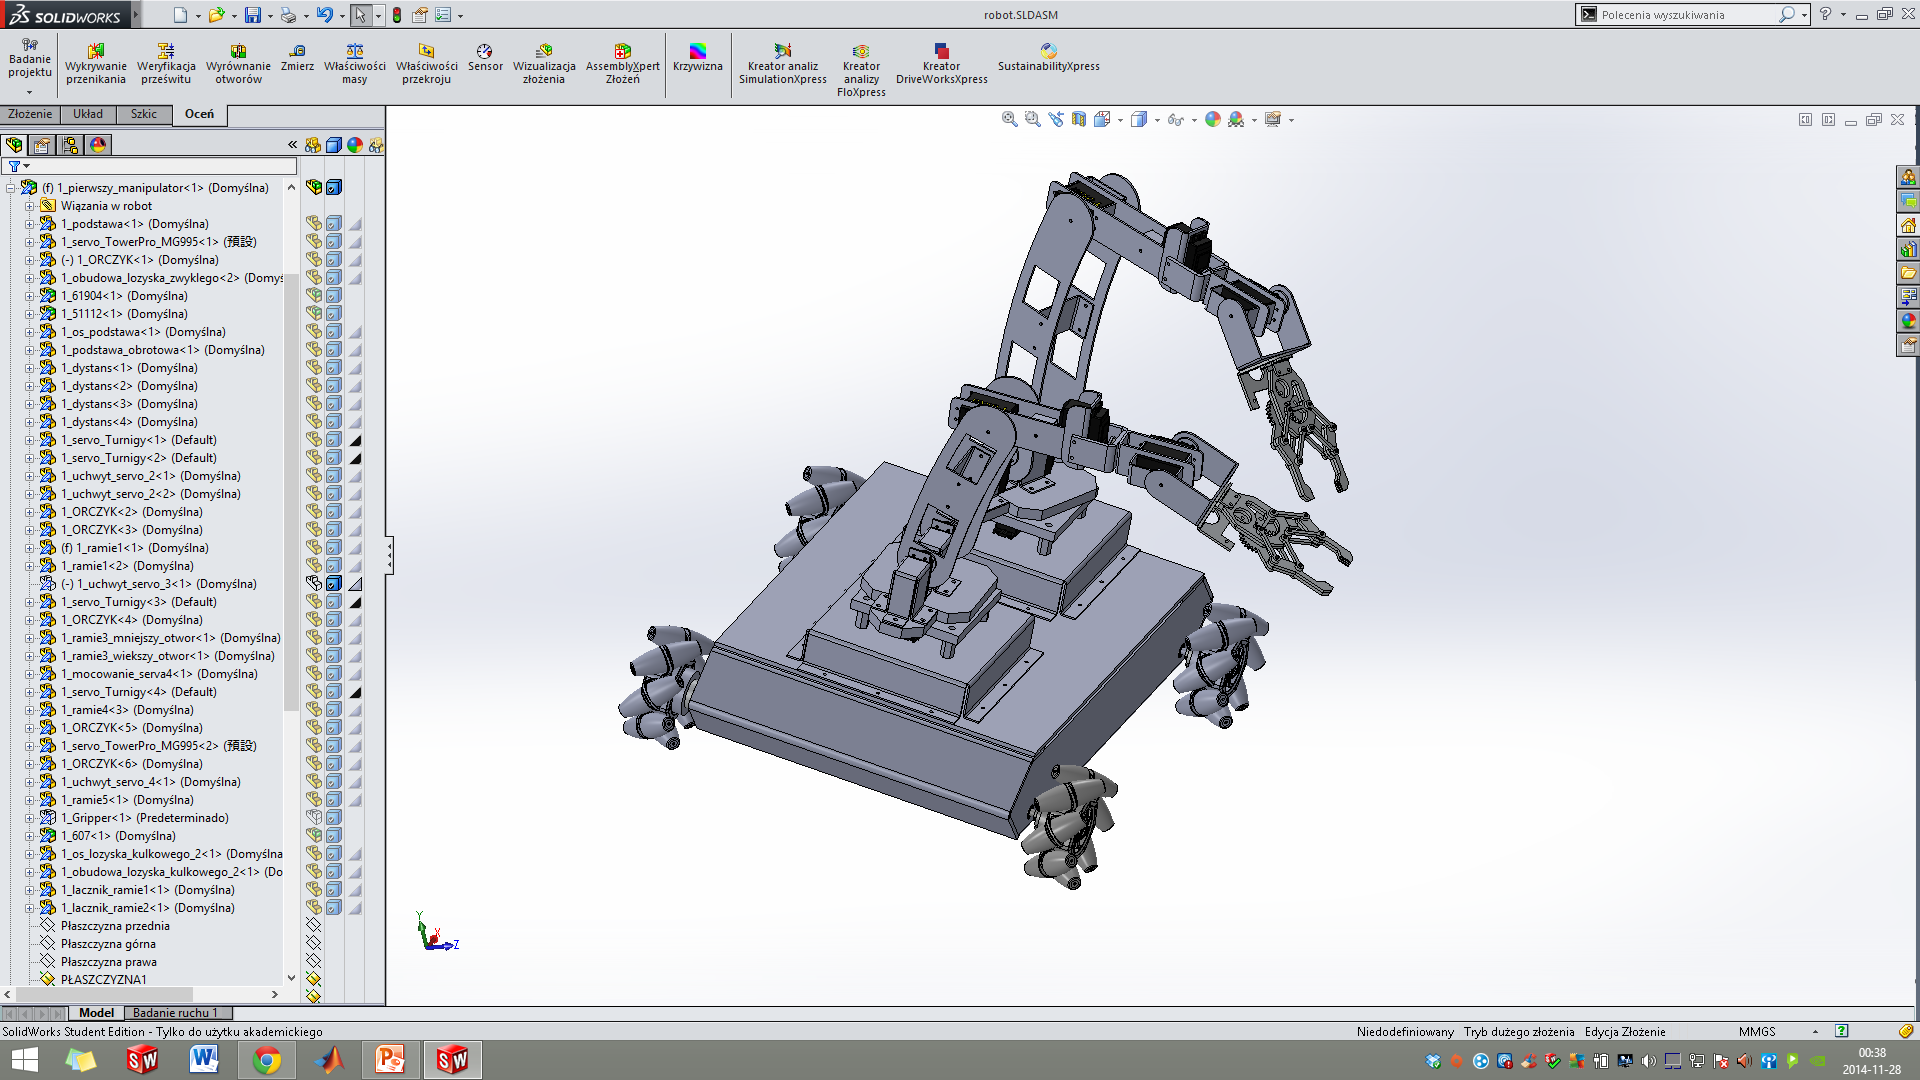
\includegraphics[trim=21cm 5cm 18cm 5cm, clip=true, totalheight=0.3\textheight]{fig/model}
\caption{Model}
\label{fig:model}
\end{figure}


The manipulators are based on a four wheeled mobile platform. To avoid complicating the mechanical design of the chassis with a steering mechanism, a special kind of wheels were used. Mecanum wheels [wikipedia], as they are called, are equipped with a set of rollers attached to their circumference at a \SI{45}{\degree} angle, which allow a vehicle to move in any direction without turning the wheels. To achieve the desired steering, the wheels are independently actuated, in a way that the resultant force vectors move or rotate the entire platform in a specified direction. In addition, such mechanism increases the stability of the entire platform, which is particularly important during the manipulation tasks. The physical dimensions of the mobile platform are also provided in the Table \ref{tab:dimensions}. The entire mechanical structure has been laser cut from aluminium sheets of \SI{1.5}{}, \SI{2}{} and \SI{4}{\milli\meter} thickness.

\begin{table}[H]

\begin{center}

\begin{tabular}{r||l}
\hline
Manipulator links  (smaller)    & 20x20 \\

\hline
Manipulator links  (bigger)        & \SI{58}{\degree H}, \SI{45}{\degree V}, \SI{70}{\degree D} \\

\hline
Mobile platform & VGA (640x480) \\

\hline
\end{tabular}
\caption{The MMS robot dimensions}
\label{tab:dimensions}
\end{center}
\end{table}


The next step in the construction of the MMS robot required a selection of hardware components, such as the actuators, power supply, embedded computing units and control electronics. The Figure \ref{fig:hardware} presents a categorized diagram of the selected elements. 

The MMS robot utilises two types of actuators, four DC motors for each of the mobile platform wheels and the servomechanisms for manipulator joints. The selected DC motors are the Pololu 1444 [datasheet] with 50:1 metal gearboxes. They achieve \SI{200}{RPM} of no-load speed and \SI{12}{\kilogram \centi\metre} of stall current. Additionally, they possess 64 CPR encoders, which multiplied by the gear ratio provide a total of 3200 counts per revolution. The type of servomechanism used for each joint, is the Turnigy 1269HV [datasheet], with titanium gears and a total stall torque of \SI{21}{\kilogram \centi\metre}. Both types of actuators are driven by the Pulse Width Modulation signal (PWM). In case of the DC motors, the PWM signal is provided by a dedicated motor driver board, named Rover 5 [datasheet]. This controller provides four low-resistance FET H-bridges, together with current monitoring on each motor channel. To generate the PWM signal for servomechanisms positioning, a 16-channel PWM driver chip, the PCA9685 [datasheet] was used. This driver has an I2C interface for setting a PWM signal on a selected channel with a 12-bit resolution.

\tikzset{
  basic/.style  = {draw, font=\sffamily, font=\footnotesize, rectangle,text centered, minimum size=2.2cm,minimum height=0.5cm},
  root/.style   = {basic, thin, align=center},
  level 2/.style = {basic, thin,align=center},
  level 3/.style = {basic, thin, align=center}
}


\begin{figure}[H]
\centering
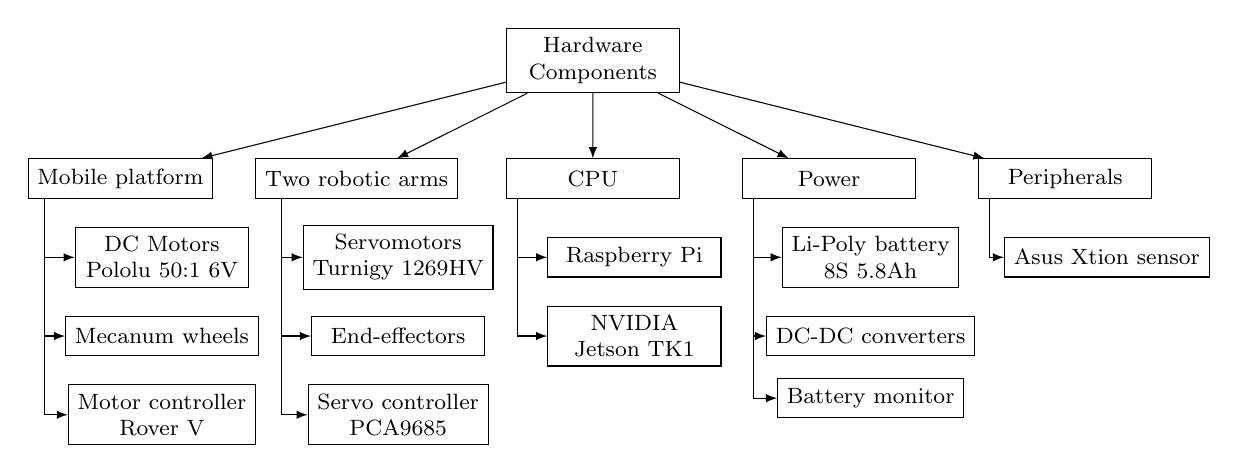
\begin{tikzpicture}[
  level 1/.style={sibling distance=30mm},
  edge from parent/.style={->,draw},
  >=latex]

% root of the the initial tree, level 1
\node[root] {Hardware\\Components}
% The first level, as children of the initial tree
  child {node[level 2] (c1) {Mobile platform}}
  child {node[level 2] (c2) {Two robotic arms}}
  child {node[level 2] (c3) {CPU}}
  child {node[level 2] (c4) {Power}}
  child {node[level 2] (c5) {Peripherals}};

% The second level, relatively positioned nodes
\begin{scope}[every node/.style={level 3}]
\node [below of = c1, xshift=15pt] (c11) {DC Motors\\ Pololu 50:1 6V};
\node [below of = c11] (c12) {Mecanum wheels};
\node [below of = c12] (c13) {Motor controller\\ Rover V};

\node [below of = c2, xshift=15pt] (c21) {Servomotors \\ Turnigy 1269HV};
\node [below of = c21] (c22) {End-effectors};
\node [below of = c22] (c23) {Servo controller\\ PCA9685};

\node [below of = c3, xshift=15pt] (c31) {Raspberry Pi};
\node [below of = c31] (c32) {NVIDIA \\ Jetson TK1};


\node [below of = c4, xshift=15pt] (c41) {Li-Poly battery \\ 8S 5.8Ah};
\node [below of = c41] (c42) {DC-DC converters};
\node [below of = c42, yshift=6pt] (c43) {Battery monitor};


\node [below of = c5, xshift=15pt] (c51) {Asus Xtion sensor};
\end{scope}

% lines from each level 1 node to every one of its "children"
\foreach \value in {1,2,3}
  \draw[->] (c1.195) |- (c1\value.west);

\foreach \value in {1,...,3}
  \draw[->] (c2.195) |- (c2\value.west);

\foreach \value in {1,...,2}
  \draw[->] (c3.195) |- (c3\value.west);
  
\foreach \value in {1,...,3}
  \draw[->] (c4.195) |- (c4\value.west);
  
\foreach \value in {1,...,1}
  \draw[->] (c5.195) |- (c5\value.west);
\end{tikzpicture}

\caption{Hardware components}
\label{fig:hardware}
\end{figure}

The main computing unit, used for hosting the control server and directly interfacing with the actuator drivers, is the model B of Raspberry Pi development platform [datasheet]. This board is equipped with 700Mhz ARM11 family CPU, 512 MB of RAM and a set of GPIO ports with hardware UART, I2C and SPI interfaces. The MMS robot utilises an additional processing unit, with a much larger computing power for the vision system implementation. The NVIDIA Jetson TK1 [datasheet] development board is based on the Tegra K1 System-on-Chip, that includes a quad-core 2.3 GHz ARM Cortex-A15 CPU, 2 GB of RAM, and a NVIDIA Kepler GPU with 192 CUDA cores, capable of performing over 300 GFLOPS of 32-bit floating point computations. This board provides a similar performance to a modern desktop GPU, while maintaining relatively low power consumption, which makes it a perfect match for image processing applications in mobile systems, such as the MMS robot.

The whole system is powered by a lithium-polymer, 8 cell battery with a nominal voltage of \SI{29.6}{\volt} and a capacity of \SI{5.8}{\ampere\hour}. Due to the specific nature of a lithium-polymer battery, each of its cells has to be protected against excessive discharge. For this purpose, a cell voltage monitor is connected to the battery, which generates a sound alarm if the voltage falls below a selected threshold. To integrate different operating voltages for the individual components, three DC-DC voltage converters are applied in the power system: one with \SI{6}{\volt} output and maximal current of \SI{20}{\ampere} for supplying all of the actuators, one with the output of \SI{12}{\volt} and \SI{4}{\ampere} max. for the NVIDIA Jetson board, and a \SI{5}{\volt} and \SI{4}{\ampere} max. for feeding the Raspberry Pi and the actuator drivers.

The final construction result in the form of the whole, assembled MMS robot is  is presented in the Figure \ref{fig:assembled}.

\begin{figure}[H]
\centering
\includegraphics[trim=15cm 18cm 28cm 10cm, clip=true, totalheight=0.3\textheight]{fig/robot}
\caption{The final effect of the MMS robot construction}
\label{fig:assembled}
\end{figure}
%---------------------------------------------------------------------------

\section{Software architecture}
\label{sec:soft}

%http://www.texample.net/tikz/examples/data-flow-diagram/
\begin{figure}[H]
\begin{center}
\begin{tikzpicture}
  [auto,every node/.style={align=center, font=\footnotesize}]
  
  \node[draw,rectangle] (manual) at (1,10) {\textbf{Manual controller} \\ (Android, PC)};
  \node[draw,circle,below right=of manual, font=\small, yshift=30pt, xshift=30pt] (raspberry) {\textbf{Control Server} \\ (Raspberry Pi)};
  \node[draw,rectangle,below left=of raspberry, yshift=45pt, xshift=-30pt] (auto) {\textbf{Autonomous mode} \\ (NVIDIA Jetson TK1)};
  \node[draw,rectangle,above right=of raspberry, yshift=-30pt, xshift=30pt] (servo) {\textbf{Servocontroller} \\ (PCA9685)};
  \node[draw,rectangle,below right=of raspberry, yshift=45pt, xshift=30pt] (motor) {\textbf{Motor controller} \\ (Rover 5)};
  %\node[draw=none,fill=none, node distance=2mm, above=of match1](ann1) {\small Recognition Pipeline for Local Descriptors};

  % draw the paths and and print some Text below/above the graph
 \path (manual) 	edge[->]  node[anchor=south,above]{HTTP}
                                    node[anchor=north,below]{WiFi} (raspberry)
(auto) 	edge[->]  node[anchor=south,above]{HTTP}
                                    node[anchor=north,below]{Ethernet} (raspberry)
 (raspberry)     	edge[->] node[anchor=south,above]{PWM} (motor)
 (raspberry)  	edge[->] node[anchor=south,above]{I2C} (servo);



  %\foreach \from/\to in {manual/raspberry,auto/raspberry,raspberry/servo,raspberry/motor}
   % \draw[->] (\from) -- (\to);

\end{tikzpicture}

\caption{Software architecture}

\label{fig:softdesign}

\end{center}
\end{figure}
